\documentclass[11pt]{article}

\usepackage{exscale}
\usepackage{graphicx}
\usepackage{amsmath}
\usepackage{latexsym}
\usepackage{times,mathptm}
\usepackage{epsfig}
\usepackage{tikz}

\textwidth 6.5truein          
\textheight 9.0truein
\oddsidemargin 0.0in
\topmargin -0.6in

\parindent 0pt          
\parskip 5pt
\def\baselinestretch{1.1}

\begin{document}

\begin{LARGE}
\centerline {\bf CSci 423 Homework 3}
\end{LARGE}
\vskip 0.25cm

\centerline{Due: 12:30 pm, Thursday, 10/3/19}
\centerline{My name}

\begin{enumerate}

\item (2, 2, 2 points) Let $\Sigma=\{a, b\}$. 
Draw state diagrams for NFAs that accept the following regular languages (given in the forms of regular expressions).
Your NFAs should use states as few as possible. 
Also, note that the ``+'' operator means one or more repetitions of the pattern.

\begin{enumerate}
\item $a(abb)^*\cup b$

\begin{center}
\begin{tikzpicture}[scale=0.2]
\tikzstyle{every node}+=[inner sep=0pt]
\draw [black] (11.7,-28.1) circle (3);
\draw (11.7,-28.1) node {$0$};
\draw [black] (29.9,-17.7) circle (3);
\draw (29.9,-17.7) node {$2$};
\draw [black] (29.9,-17.7) circle (2.4);
\draw [black] (45.6,-17.7) circle (3);
\draw (45.6,-17.7) node {$3$};
\draw [black] (59.5,-17.7) circle (3);
\draw (59.5,-17.7) node {$4$};
\draw [black] (29.8,-41.1) circle (3);
\draw (29.8,-41.1) node {$1$};
\draw [black] (29.8,-41.1) circle (2.4);
\draw [black] (14.3,-26.61) -- (27.3,-19.19);
\fill [black] (27.3,-19.19) -- (26.35,-19.15) -- (26.85,-20.02);
\draw (21.74,-23.4) node [below] {$a$};
\draw [black] (14.14,-29.85) -- (27.36,-39.35);
\fill [black] (27.36,-39.35) -- (27.01,-38.48) -- (26.42,-39.29);
\draw (19.75,-35.1) node [below] {$b$};
\draw [black] (32.9,-17.7) -- (42.6,-17.7);
\fill [black] (42.6,-17.7) -- (41.8,-17.2) -- (41.8,-18.2);
\draw (37.75,-18.2) node [below] {$a$};
\draw [black] (48.6,-17.7) -- (56.5,-17.7);
\fill [black] (56.5,-17.7) -- (55.7,-17.2) -- (55.7,-18.2);
\draw (52.55,-18.2) node [below] {$b$};
\draw [black] (31.392,-15.102) arc (144.8486:35.1514:16.276);
\fill [black] (31.39,-15.1) -- (32.26,-14.74) -- (31.44,-14.16);
\draw (44.7,-7.7) node [above] {$b$};
\draw [black] (6.7,-35.3) -- (9.99,-30.56);
\fill [black] (9.99,-30.56) -- (9.12,-30.94) -- (9.94,-31.51);
\end{tikzpicture}
\end{center}

\item $a^+\cup (ab)^+$

\begin{center}
\begin{tikzpicture}[scale=0.2]
\tikzstyle{every node}+=[inner sep=0pt]
\draw [black] (11.9,-28.6) circle (3);
\draw (11.9,-28.6) node {$0$};
\draw [black] (35.2,-16.9) circle (3);
\draw (35.2,-16.9) node {$1$};
\draw [black] (35.2,-16.9) circle (2.4);
\draw [black] (35.2,-36.2) circle (3);
\draw (35.2,-36.2) node {$2$};
\draw [black] (55.6,-36.2) circle (3);
\draw (55.6,-36.2) node {$3$};
\draw [black] (55.6,-36.2) circle (2.4);
\draw [black] (14.58,-27.25) -- (32.52,-18.25);
\fill [black] (32.52,-18.25) -- (31.58,-18.16) -- (32.03,-19.05);
\draw (24.49,-23.25) node [below] {$a$};
\draw [black] (34.49,-13.997) arc (221.47119:-66.52881:2.25);
\draw (37.27,-9.73) node [above] {$a$};
\fill [black] (37.07,-14.57) -- (38,-14.42) -- (37.34,-13.67);
\draw [black] (14.75,-29.53) -- (32.35,-35.27);
\fill [black] (32.35,-35.27) -- (31.74,-34.55) -- (31.43,-35.5);
\draw (22.72,-32.94) node [below] {$a$};
\draw [black] (54.249,-38.868) arc (-34.8233:-145.1767:10.78);
\fill [black] (54.25,-38.87) -- (53.38,-39.24) -- (54.2,-39.81);
\draw (45.4,-43.99) node [below] {$b$};
\draw [black] (36.764,-33.651) arc (140.7602:39.2398:11.15);
\fill [black] (36.76,-33.65) -- (37.66,-33.35) -- (36.88,-32.71);
\draw (45.4,-29.05) node [above] {$a$};
\end{tikzpicture}
\end{center}

\item $(a\cup b^+)a^+b^+$

\begin{center}
\begin{tikzpicture}[scale=0.2]
\tikzstyle{every node}+=[inner sep=0pt]
\draw [black] (7.1,-28.5) circle (3);
\draw (7.1,-28.5) node {$0$};
\draw [black] (24.2,-16.4) circle (3);
\draw (24.2,-16.4) node {$1$};
\draw [black] (23.8,-38.4) circle (3);
\draw (23.8,-38.4) node {$3$};
\draw [black] (45.5,-27.8) circle (3);
\draw (45.5,-27.8) node {$2$};
\draw [black] (63.2,-39) circle (3);
\draw (63.2,-39) node {$4$};
\draw [black] (63.2,-39) circle (2.4);
\draw [black] (9.55,-26.77) -- (21.75,-18.13);
\fill [black] (21.75,-18.13) -- (20.81,-18.19) -- (21.39,-19);
\draw (16.6,-22.95) node [below] {$a$};
\draw [black] (9.68,-30.03) -- (21.22,-36.87);
\fill [black] (21.22,-36.87) -- (20.79,-36.03) -- (20.28,-36.89);
\draw (14.45,-33.95) node [below] {$b$};
\draw [black] (25.123,-41.08) arc (54:-234:2.25);
\draw (23.8,-45.65) node [below] {$b$};
\fill [black] (22.48,-41.08) -- (21.6,-41.43) -- (22.41,-42.02);
\draw [black] (26.5,-37.08) -- (42.8,-29.12);
\fill [black] (42.8,-29.12) -- (41.87,-29.02) -- (42.31,-29.92);
\draw (35.58,-33.61) node [below] {$a$};
\draw [black] (26.84,-17.82) -- (42.86,-26.38);
\fill [black] (42.86,-26.38) -- (42.39,-25.57) -- (41.91,-26.45);
\draw (35.79,-21.6) node [above] {$a$};
\draw [black] (44.966,-24.86) arc (218.02347:-69.97653:2.25);
\draw (48.12,-20.76) node [above] {$a$};
\fill [black] (47.51,-25.59) -- (48.45,-25.49) -- (47.83,-24.7);
\draw [black] (48.04,-29.4) -- (60.66,-37.4);
\fill [black] (60.66,-37.4) -- (60.26,-36.55) -- (59.72,-37.39);
\draw (53.35,-33.9) node [below] {$b$};
\draw [black] (62.429,-36.113) arc (222.69007:-65.30993:2.25);
\draw (65.08,-31.79) node [above] {$b$};
\fill [black] (65.02,-36.63) -- (65.95,-36.46) -- (65.27,-35.72);
\end{tikzpicture}
\end{center}

\end{enumerate}

Collaborators: Ethan Young, Will Elliot and Yang Zhang

\item (5 points) Let $R_1$ and $R_2$ be any regular expressions. For each identity below, decide True or False.
\begin{enumerate}
\item $(R_1\cup R_2)^* = R_1^*\cup R_2^*$
\item $(R_1R_2\cup R_1)^*R_1 = R_1(R_2R_1\cup R_1)^*$
\item $(R_1R_2\cup R_1)^*R_1R_2 = (R_1R_1^*R_2)^*$ 
\item $(R_1\cup R_2)^*R_2 = (R_1^*R_2)^*$
\item $R_2(R_1R_2\cup R_2)^*R_1 = R_1R_1^*R_2(R_1R_1^*R_2)^*$ 
\end{enumerate}

Soultion:
\begin{enumerate}
\item F
\item T
\item F
\item F
\item F
\end{enumerate}

Collaborators: Ethan Young, Will Elliot and Yang Zhang

\item (3, 5 points) Regular expressions and languages.
\begin{enumerate}
\item Let $L_1=\{w\in\{0,1\}^* | w{\rm\ has\ no\ pair\ of\ consecutive\ zeros}\}$. Give a simple regular expression for $L_1$. 
\item Let $L_2=\{w\in\{0,1\}^* | w{\rm\ does\ not\ have\ 101\ as\ a\ substring}\}$. Give a simple regular expression for $L_2$.
\end{enumerate}

Solution:

\begin{enumerate}
\item $(1^{+}0)^{*} \cup (01^{*})^{*} \cup (1^{+}01^{*})^{*} $
\item $(0^{*}1^{*}0^{+}0^{+}1^{*})^{*}0^{*} \cup 0^{*}1^{*} \cup 1^{*}0^{*}$
\end{enumerate}

Collaborators: Ethan Young, Will Elliot and Yang Zhang

\item (3, 3 points) Let $\Sigma=\{a, b\}$.
Let $D$ be a language of strings that contain an even number of $a$'s and an odd number of $b$'s and do not contain the substring $ab$.

\begin{enumerate}
\item Given a simple regular expression for $D$.
\item Draw the state diagram for the DFA with no more than five states.
\end{enumerate}

Solution
\begin{enumerate}
\item $b(bb)^{*}(aa)^{*}$
\item 
\begin{center}
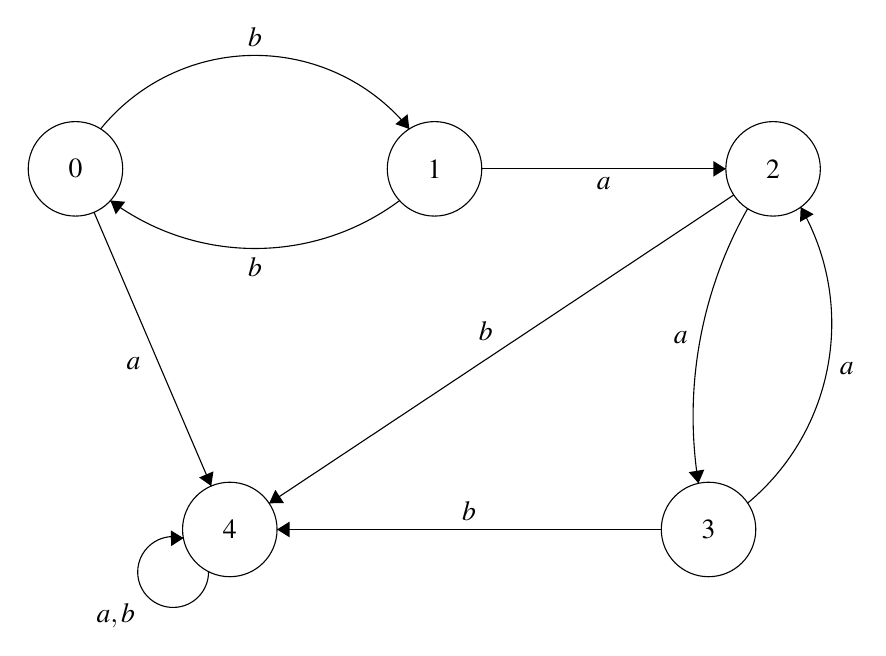
\begin{tikzpicture}[scale=0.2]
\tikzstyle{every node}+=[inner sep=0pt]
\draw [black] (12.5,-15.7) circle (3);
\draw (12.5,-15.7) node {$0$};
\draw [black] (35.3,-15.7) circle (3);
\draw (35.3,-15.7) node {$1$};
\draw [black] (56.8,-15.7) circle (3);
\draw (56.8,-15.7) node {$2$};
\draw [black] (52.7,-38.6) circle (3);
\draw (52.7,-38.6) node {$3$};
\draw [black] (22.3,-38.6) circle (3);
\draw (22.3,-38.6) node {$4$};
\draw [black] (14.096,-13.168) arc (140.95917:39.04083:12.622);
\fill [black] (33.7,-13.17) -- (33.59,-12.23) -- (32.81,-12.86);
\draw (23.9,-8) node [above] {$b$};
\draw [black] (33.083,-17.714) arc (-53.32532:-126.67468:15.376);
\fill [black] (14.72,-17.71) -- (15.06,-18.59) -- (15.66,-17.79);
\draw (23.9,-21.26) node [below] {$b$};
\draw [black] (38.3,-15.7) -- (53.8,-15.7);
\fill [black] (53.8,-15.7) -- (53,-15.2) -- (53,-16.2);
\draw (46.05,-16.2) node [below] {$a$};
\draw [black] (52.059,-35.671) arc (-170.86517:-209.43612:26.831);
\fill [black] (52.06,-35.67) -- (52.43,-34.8) -- (51.44,-34.96);
\draw (51.42,-26.42) node [left] {$a$};
\draw [black] (58.548,-18.132) arc (29.91869:-50.21999:14.83);
\fill [black] (58.55,-18.13) -- (58.51,-19.07) -- (59.38,-18.58);
\draw (61.01,-28.4) node [right] {$a$};
\draw [black] (54.3,-17.36) -- (24.8,-36.94);
\fill [black] (24.8,-36.94) -- (25.74,-36.92) -- (25.19,-36.08);
\draw (38.55,-26.65) node [above] {$b$};
\draw [black] (49.7,-38.6) -- (25.3,-38.6);
\fill [black] (25.3,-38.6) -- (26.1,-39.1) -- (26.1,-38.1);
\draw (37.5,-38.1) node [above] {$b$};
\draw [black] (13.68,-18.46) -- (21.12,-35.84);
\fill [black] (21.12,-35.84) -- (21.26,-34.91) -- (20.35,-35.3);
\draw (16.67,-28.1) node [left] {$a$};
\draw [black] (20.95,-41.266) arc (0.8699:-287.1301:2.25);
\draw (16.32,-44.05) node [left] {$a,b$};
\fill [black] (19.36,-39.15) -- (18.56,-38.66) -- (18.57,-39.66);
\end{tikzpicture}
\end{center}
\end{enumerate}


Collaborators: Ethan Young, Will Elliot and Yang Zhang

\item (5 points) Let $A=\{w\in\{0, 1\}^* |\ w {\rm\ is\ a\ binary\ number\ that\ is\ a\ multiple\ of\ }5\}$. 
Prove that $A$ is regular by giving the state diagram of a DFA that accepts $A$.

\begin{center}
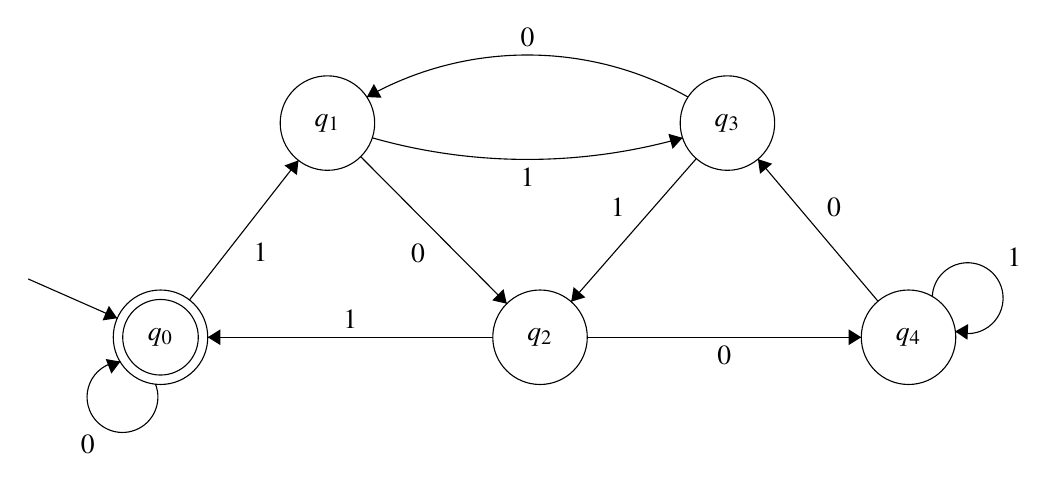
\begin{tikzpicture}[scale=0.2]
\tikzstyle{every node}+=[inner sep=0pt]
\draw [black] (22.2,-21.4) circle (3);
\draw (22.2,-21.4) node {$q_1$};
\draw [black] (47.6,-21.4) circle (3);
\draw (47.6,-21.4) node {$q_3$};
\draw [black] (11.6,-35) circle (3);
\draw (11.6,-35) node {$q_0$};
\draw [black] (11.6,-35) circle (2.4);
\draw [black] (35.7,-35) circle (3);
\draw (35.7,-35) node {$q_2$};
\draw [black] (59.1,-35) circle (3);
\draw (59.1,-35) node {$q_4$};
\draw [black] (11.277,-37.971) arc (21.52881:-266.47119:2.25);
\draw (6.98,-41.19) node [below] {$0$};
\fill [black] (9.05,-36.55) -- (8.12,-36.38) -- (8.48,-37.31);
\draw [black] (13.44,-32.63) -- (20.36,-23.77);
\fill [black] (20.36,-23.77) -- (19.47,-24.09) -- (20.26,-24.7);
\draw (17.47,-29.61) node [right] {$1$};
\draw [black] (24.31,-23.53) -- (33.59,-32.87);
\fill [black] (33.59,-32.87) -- (33.38,-31.95) -- (32.67,-32.66);
\draw (28.43,-29.68) node [left] {$0$};
\draw [black] (44.751,-22.338) arc (-74.15593:-105.84407:36.083);
\fill [black] (44.75,-22.34) -- (43.85,-22.08) -- (44.12,-23.04);
\draw (34.9,-24.21) node [below] {$1$};
\draw [black] (38.7,-35) -- (56.1,-35);
\fill [black] (56.1,-35) -- (55.3,-34.5) -- (55.3,-35.5);
\draw (47.4,-35.5) node [below] {$0$};
\draw [black] (32.7,-35) -- (14.6,-35);
\fill [black] (14.6,-35) -- (15.4,-35.5) -- (15.4,-34.5);
\draw (23.65,-34.5) node [above] {$1$};
\draw [black] (24.7,-19.747) arc (119.34601:60.65399:20.812);
\fill [black] (24.7,-19.75) -- (25.64,-19.79) -- (25.15,-18.92);
\draw (34.9,-16.58) node [above] {$0$};
\draw [black] (45.62,-23.66) -- (37.68,-32.74);
\fill [black] (37.68,-32.74) -- (38.58,-32.47) -- (37.83,-31.81);
\draw (41.11,-26.75) node [left] {$1$};
\draw [black] (57.16,-32.71) -- (49.54,-23.69);
\fill [black] (49.54,-23.69) -- (49.67,-24.62) -- (50.44,-23.98);
\draw (53.9,-26.76) node [right] {$0$};
\draw [black] (60.607,-32.419) arc (177.45531:-110.54469:2.25);
\draw (65.34,-29.95) node [right] {$1$};
\fill [black] (62.06,-34.63) -- (62.84,-35.16) -- (62.89,-34.16);
\draw [black] (3.2,-31.3) -- (8.85,-33.79);
\fill [black] (8.85,-33.79) -- (8.32,-33.01) -- (7.92,-33.93);
\end{tikzpicture}
\end{center}

Collaborators: Ethan Young, Will Elliot and Yang Zhang

\end{enumerate}

\end{document}